\documentclass[fleqn]{article}

\usepackage{polski}
\usepackage[utf8]{inputenc}
\usepackage[polish]{babel}
\usepackage{parskip}
\usepackage{icomma}
\usepackage[a4paper,includeheadfoot,margin=1.27cm]{geometry}
\usepackage{float}
\usepackage{graphicx}
\usepackage{amsmath}
\usepackage[hypcap=true]{subcaption}
\usepackage{xcolor}
\usepackage{transparent}
\usepackage{listings}
\usepackage[colorlinks=true, linkcolor=blue, pdfborder={0 0 0}]{hyperref}

\renewcommand\thesection{\arabic{section}.}
\renewcommand\thesubsection{\alph{subsection})}
\renewcommand\thesubsubsection{}
\newcommand\square[1]{
	\fcolorbox{black}{#1}{\rule{0pt}{6pt}\rule{6pt}{0pt}}
}

\brokenpenalty=1000
\clubpenalty=1000
\widowpenalty=1000

\lstdefinestyle{customc}{
	belowcaptionskip=1\baselineskip,
	breaklines=true,
	frame=L,
	xleftmargin=\parindent,
	language=C,
	showstringspaces=false,
	basicstyle=\footnotesize\ttfamily,JESTEM JESTEM
	keywordstyle=\bfseries\color{green!40!black},
	commentstyle=\itshape\color{purple!40!black},
	identifierstyle=\color{blue},
	stringstyle=\color{orange},
}

\title{TM -- Laboratorium 4. \\ \large Minutnik dynamiczny}
\author{Krystian Chachuła \\ Dawid Gruszczyński \\ Marcin Skrzypkowski}

\begin{document}

\maketitle

\setcounter{page}{0}
\thispagestyle{empty}

\pagebreak

\setcounter{page}{1}

\section{Wstęp}

Naszym zadaniem na czwartym laboratorium było zaprojektowanie i zrealizowanie minutnika na platformie MSP430 w języku C. Czas miał być zadawany przez przyciski monostabilne, kolejnym założeniem było dołączenie dodatkowej funkcjonalności wzbogacającej działanie systemu oraz zapewniającej intuicyjne działanie.

Ostateczny układ składał się z następujących elementów:

\begin{itemize}
	\item \textbf{10\_PS1} (moduł zasilacza)
	\item \textbf{570\_MSP430F14x} (moduł mikrokontrolera Texas Instruments serii MSP430f14x lub F16x)
	\item \textbf{120\_IN8} (zestaw 8 monostabilnych wyłączników)
	\item \textbf{411\_WYS-DYN} (moduł wyświetlacza dynamicznego)
	\item \textbf{007\_TBD} (moduł głośnika ze wzmacniaczem)
\end{itemize}

\section{Implementacja}

Rozpoczęliśmy projektowanie od podziału zadania na mniejsze bloki, aby uzyskać większy komfort pracy i ułatwić orientację. Stowrzyliśmy więc pliki służące do obsługi przycisków, wyświetlania symboli, podstawowych funkcji minutnika oraz odtwarzania melodii. Cały algorytm jednak został zaimplementowany w pliku main.


\section{Wyświetlanie}

Ponieważ wyświetlacz dynamiczny, z którego korzystaliśmy w tym ćwiczeniu, ma możliwość wyświetlania tylko jendego symbolu na raz, musieliśmy przełączać się między kolejnymi znakami. W tym celu najpierw musieliśmy mieć możliwość manipulacji częstotliwością. Do odliczania jednej sekundy, która była również potrzebna do wykonania zadania minutnika (założyliśmy dokładność jednej sekundy), wykorzystaliśmy zegar ACLK ustawiony na częstotliwość $32.768$ kHz. Korzystając z tego, że timery w MSP430 są 16-bitowe, mogliśmy wykorzystać jeden kanał timera A do odliczania pełnych sekund. W celu sprawdzenia, czy wybrany przez nas sposób mierzenia czasu jest dopuszczalny, sprawdziliśmy częstotliwość generowania przerwań kanału na oscyloskopie. Poniżej znajdują się wyniki testów.

\begin{figure}[H]
	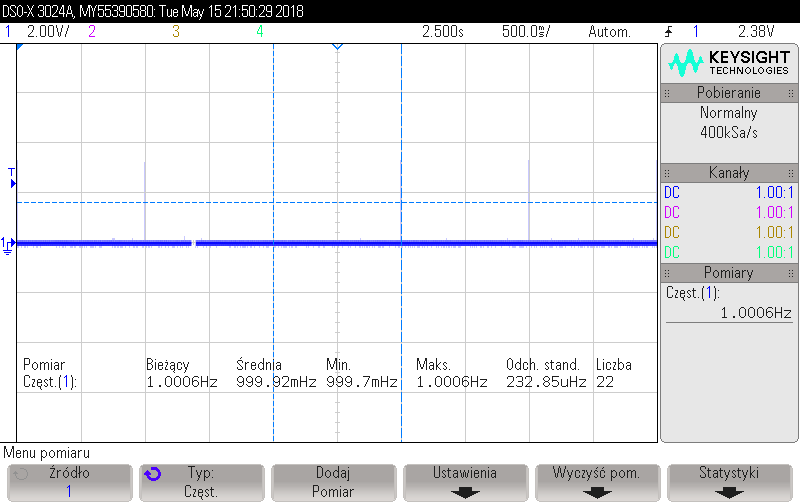
\includegraphics[width=\textwidth]{scope_1.png}
	\caption{Test odliczania jednej sekundy na wybranej przez nas częstotliwości $32.768 kHz$}
\end{figure}

Po 20 próbkach odchylenie standardowe od jednej sekundy wynosiło $232.85$ $\mu$s, stwierdziliśmy że jest to wystarczająca dokładność do zrealizowania naszego zadania.

Ostateczna postać minutnika posiadała pięć symboli, 2 cyfry odpowiedzialne za wyświetlanie minut (więc maksymalną wartością do ustawienia było $99:59$) oraz jeden symbol oznaczający tryb, w którym aktualnie znajduje się minutnik.



































































% DAWID WORKSPACE


\section{Usprawnienia oraz niezbędne modyfikacje projektu}
Minutnik wzbogaciliśmy o kilka dodatkowych funkcjonalności. Są to między innymi sygnalizacja trybu w jakim aktualnie się znajduje, zerowanie zawartości oddzielnym przyciskiem oraz odgrywanie melodii sygnalizujacej zakończenie odliczania.

Sygnalizacja trybu pracy odbywa się poprzez wyświetlanie na jednym z wyświetlaczy siedmiosegmentowych litery t gdy minutnik jest w trakcie odliczania lub litery c podczas gdy jest zatrzymany lub ustawiany jest czas zliczania.

Przycisk zerujący dodaliśmy w celu umożliwienia łatwego i szybkiego zerowania minutnika. Pozwala on także na wyłączenie alarmu sygnalizującego zliczanie.

Największym usprawnieniem minutnika jest odgrywanie melodii sygnalizującej zakończenie odliczania. Odbywa się to poprzez generację odpowiednio skofnigurowanego sygnału PWM oraz odtwarzanie go za pomocą modułu głośniczka ze wzmacniaczem. Do ogdrywania melodii służy klasa Synth, która przechowuje interwały oraz częstotliwości każdej nuty, natomiast sygnał PWM generowany jest

\pagebreak

\section{Program}
\subsection{main.c}

\noindent\begin{minipage}[t]{.45\textwidth}
	\lstinputlisting[lastline=64, style=customc]{src/main.c}
\end{minipage}\hfill
\noindent\begin{minipage}[t]{.45\textwidth}
	\lstinputlisting[firstline=65, lastline=119, style=customc]{src/main.c}
\end{minipage}\hfill
\pagebreak

\noindent\begin{minipage}[t]{.45\textwidth}
	\lstinputlisting[firstline=121, lastline=180, style=customc]{src/main.c}
\end{minipage}\hfill
\noindent\begin{minipage}[t]{.45\textwidth}
	\lstinputlisting[firstline=181, style=customc]{src/main.c}
	\subsection{Buttons}
	\subsubsection{Buttons.h}
	\lstinputlisting[style=customc]{src/Buttons.h}
	\subsubsection{Buttons.c}
	\lstinputlisting[style=customc]{src/Buttons.c}
\end{minipage}\hfill

\pagebreak

\subsection{Lcd}

\noindent\begin{minipage}[t]{.45\textwidth}
	\subsubsection{Lcd.h}
	\lstinputlisting[style=customc]{src/Lcd.h}
\end{minipage}\hfill
\noindent\begin{minipage}[t]{.45\textwidth}
	\subsubsection{Lcd.c}
	\lstinputlisting[style=customc]{src/Lcd.c}
\end{minipage}\hfill

\pagebreak

\noindent\begin{minipage}[t]{.45\textwidth}
\subsection{CtdnTimer}
\subsubsection{CtdnTimer.h}
\lstinputlisting[style=customc]{src/CtdnTimer.h}
\subsubsection{CtdnTimer.c}
\lstinputlisting[style=customc]{src/CtdnTimer.c}
\end{minipage}\hfill
\noindent\begin{minipage}[t]{.45\textwidth}
\subsection{melodies.h}
\lstinputlisting[style=customc]{src/melodies_slim.h}
\end{minipage}\hfill

\pagebreak

\section{Możliwości udoskonalenia systemu}
Możliwym udoskonaleniem

\end{document}
\grid
